
Ici sont résumés les travaux futures concernant l'implémentation 
ou le projet de façon plus générale.

\subsection{code} % (fold)
\label{sub:code}
Concernant le code quelques fonctionnalités peuvent être ajoutées:
\begin{itemize}
	\item Des tests de l'implémentation
	\item La fonction rendant la représentation intermédiaire
	\item le clonage des poids pour les réseaux siamois
	\item Implémenter la Reverse (Cross) Validation
\end{itemize}

De plus il serait judicieux d'ajouter aux exemples les graphiques obtenus
par une \href{http://scikit-learn.org/stable/modules/generated/sklearn.manifold.TSNE.html}{TSNE}.

% subsection code (end)
\subsection{Calibration} % (fold)
\label{sub:calibration}

Afin de valider l'implémentation du DANN mais aussi de commencer à travailler
sur le problème de calibration/correction la prochaine étape consistera à 
chercher à accrocher un DANN sur un auto-encodeur afin de chercher à inverser
une transformation des données pour obtenir une représentation commune restant
dans l'espace d'origine.

On a ainsi deux domaines: 
les données originelles $X_S$ et les données transformées $X_T = \phi(X_S)$.
On souhaite apprendre une représentation commune. Cependant les contraintes 
d'interprétabilité impose que l'on laisse les données originelle tel quel et 
que l'on se contente de corriger les données transformées pour les ramener sur
leur distribution d'origine.

Ainsi l'auto-encodeur va coder les données transformées mais ignorer les données
originelle. Puis le décodeur aura pour tâche d'apprendre à retrouver les données
transformées tout en essayant d'apprendre l'identité pour les données originelles.
Enfin le DANN forcera la représentation intermédiaire, ici les données codées, à
être aussi proche que possible.

La structure est représentée figure \ref{fig:AutoDANN}.

\begin{figure*}[htbp]
\centering
\subfigure[Auto-DANN conceptuel.]
	{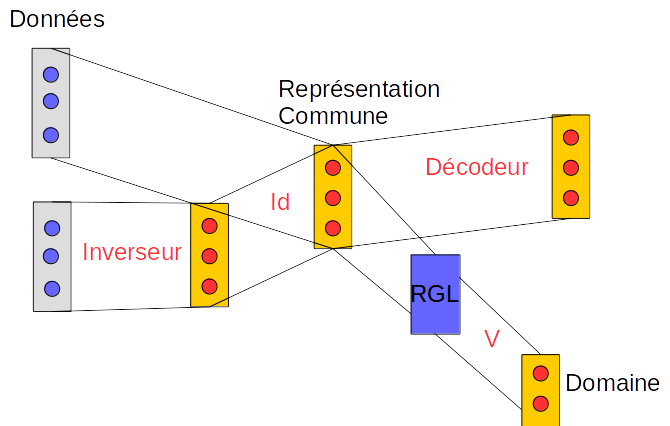
\includegraphics[width=\columnwidth]{fig/AutoDANN.png}}
\caption{Auto-DANN du point vue conceptuel.}
\label{fig:AutoDANNC}

\subfigure[Auto-DANN propagation avant.]
	{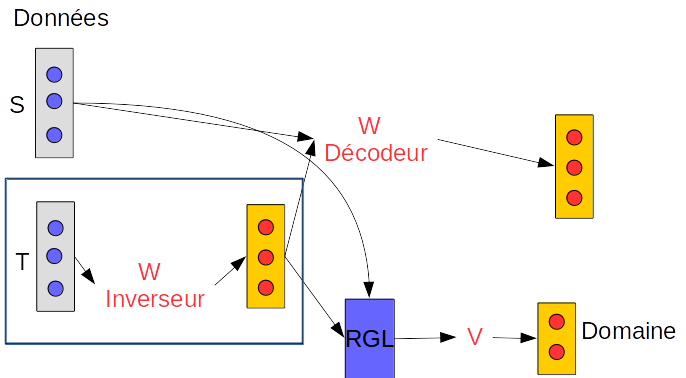
\includegraphics[width=\columnwidth]{fig/AutoDANNLasagne.png}}
\hfill
\subfigure[Auto-DANN propagation arrière.]
	{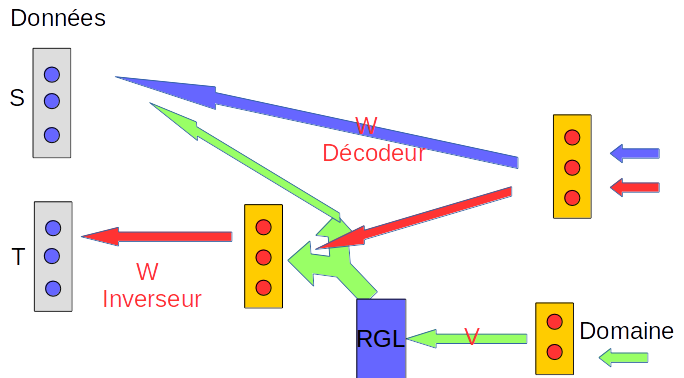
\includegraphics[width=\columnwidth]{fig/AutoDANNBackprop.png}}
\caption{Auto-DANN du point vue de l'implémentation.}
\label{fig:AutoDANN}
\end{figure*}

Remarque:
Ce qui m'inquiète un peu c'est qu'on a pas que DANN vs Auto-encodeur
mais aussi Source-décodeur vs Cible-décodeur... Bon après c'est pas dis que ça
va mal se passer.

% subsection calibration (end)
\subsection{Expériences} % (fold)
\label{sub:experiences}

Parmi les expériences possibles SVHN vs MNIST est un problème qui doit être
exploré dans un future proche j'espère.

% subsection expériences (end)
